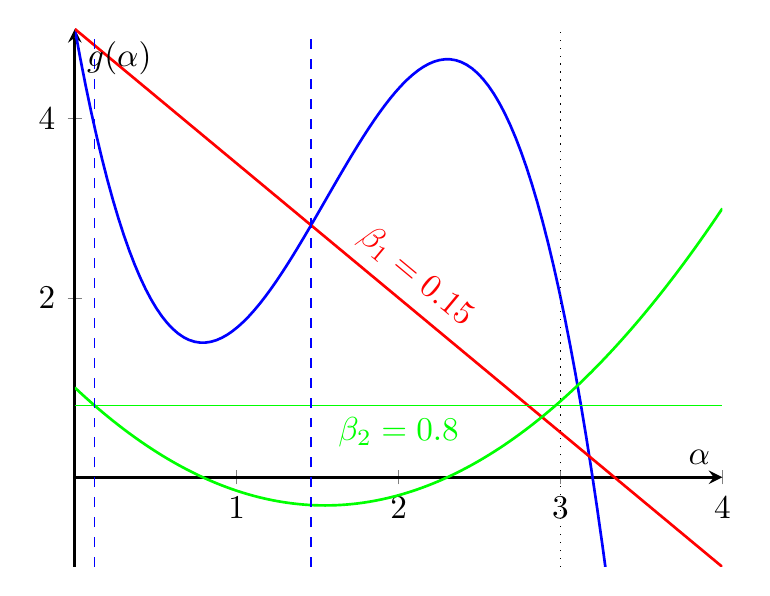
\begin{tikzpicture}[scale=1.2]
  \begin{axis}[
      xlabel={$\alpha$},
      ylabel={$g(\alpha)$}, 
      axis y line=middle,   
      axis x line=middle,   
      samples=120,
      thick,
      xmin=0,
      xmax=4,
      domain=0:4,
      ymin=-1,
      ymax=5
    ]
    \addplot+[mark=none, color=blue, thick]{-1.833 * x*x*x + 8.5 * x * x - 10 * x + 5};
    \addplot+[mark=none, color=red, thick]{5-0.15*10*x} node[pos=0.5, above, sloped] (A) {$\beta_1=0.15$};
    \addplot+[mark=none, color=black, thin, dotted] coordinates {(3, -1) (3, 5)} ;
    \addplot+[mark=none, color=green, thick, domain=0:4]{(-1.833*3*x*x + 2*8.5 * x -10)/-10};
    \addplot+[mark=none, color=green, thin] coordinates {(0, 0.8) (4, 0.8)}
      node[pos=0.5, below] (B) {$\beta_2=0.8$};
    \addplot +[mark=none, color=blue, thin, dashed] coordinates {(0.1225, -1) (0.1225, 5)} ;
    \addplot +[mark=none, color=blue, thin, dashed] coordinates {(1.45912, -1) (1.45912, 5)} ;
  \end{axis}
\end{tikzpicture}
